\newpage
\section{User}

\subsection{How does it work?}

In the Salespointframework there is one \code{PersistentUsermanger}, but it is not a singleton. You can instantiate a new
\code{PersistentUsermanger} whenever you need it (it always manages the same data!).
The \code{UserManger} is the main part of the \code{user}-package. It connects all parts:
You can add and remove users to/from the system and also add and remove \code{UserCapability}s of the users in the system.

\begin{figure}[ht]
	\centering
  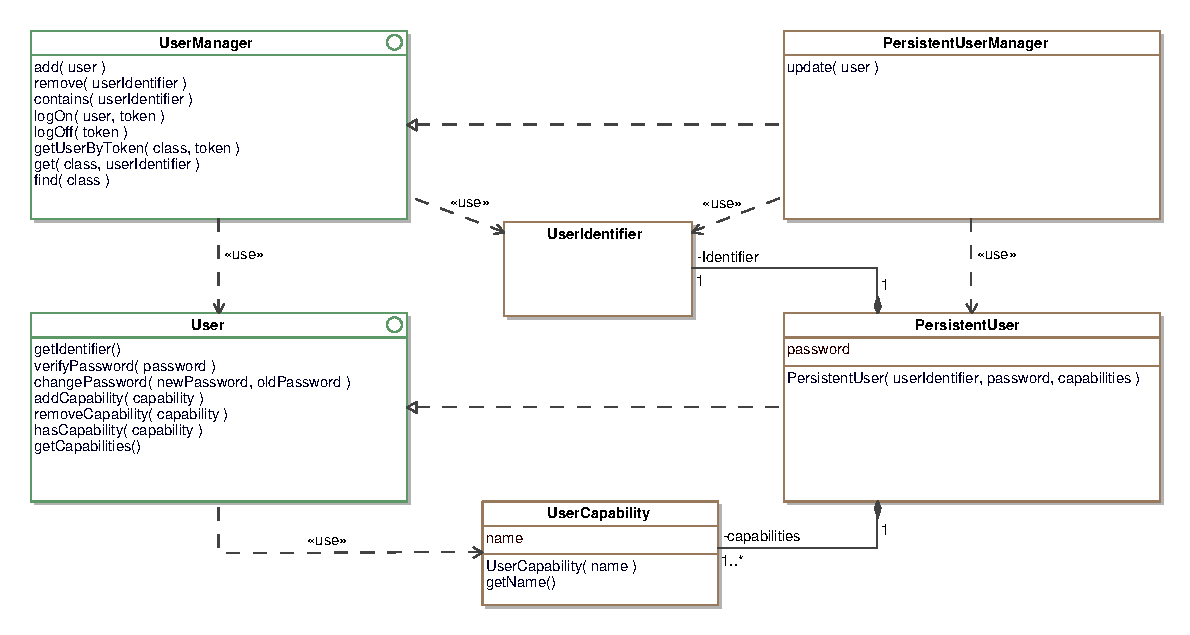
\includegraphics[width=1.0\textwidth]{images/User_Overview.eps}
	\label{user_overview}
	\caption{User - Class Overview}
\end{figure}

\subsection{Ensure correct data}
To ensure you have the correct data in your system you should only access users and their capabilities via the \code{PersistentUsermanger}:

During the process of adding a user to the system the \code{PersistentUsermanger} ensures that there will be no duplicate users. If you try to add a \code{User} with an \code{UserIdentifier} that is already in the system a \code{DuplicateUserException} will be thrown. This will help you to identify \code{Users} correctly, e.g. during the login process.

You should notice that it is not possible to remove users with open \code{Order}s! You have to close/finish them before.

You are only able to add a \code{UserCapability} to a \code{User}, who is in they system. Otherwise you will get an \code{UnknownUserException}.
This ensures that a new \code{User} will have no \code{UserCapabilities}.

\subsection{Why are there so many users?}
First of all we do have the \code{User} interface. This provides all basic methods. There is an implementation of it: The
\code{PersistentUser} class which also has the basic attributes of an user.

\subsection{Login}

ASK PAUL!





